\documentclass[aspectratio=169]{beamer}
\usepackage{amsmath, amssymb, amsfonts, amsthm}
\usepackage{cancel}
\usepackage[output-complex-root=j]{siunitx}
\usepackage[american, nooldvoltagedirection]{circuitikz}
\usepackage{bm}
\usepackage{listings}
\usepackage{graphicx}
\usepackage{hyperref}

\usetheme{Berkeley}
\usefonttheme[onlymath]{serif}
\AtBeginSection[]{
    \begin{frame}
    \vfill
    \centering
    \begin{beamercolorbox}[sep=8pt,center,shadow=false,rounded=false]{title}
    \usebeamerfont{title}\insertsectionhead\par
    \end{beamercolorbox}
    \vfill
    \end{frame}
}

\newcommand{\N}{\mathbb{N}}
\newcommand{\Z}{\mathbb{Z}}
\newcommand{\Q}{\mathbb{Q}}
\newcommand{\R}{\mathbb{R}}
\newcommand{\C}{\mathbb{C}}
\newcommand{\tpose}[1]{#1^\top}
\newcommand{\diff}[1]{\frac{d}{d #1}}

\title{EECS 16B CSM}
\author{Bryan Ngo}
\date{2022-04-19}
\institute{UC Berkeley}

\begin{document}

\begin{frame}
    \maketitle
\end{frame}

\begin{frame}
    \tableofcontents
\end{frame}

\section{PCA}

\begin{frame}
    \frametitle{PCA}

    \begin{itemize}
        \item allows us to reduce dimensionality
        \item preserve only most important singular components
    \end{itemize}
\end{frame}

\begin{frame}
    \frametitle{PCA}
    \framesubtitle{Steps}

    \begin{enumerate}
        \item do SVD
        \item pick the first \(\sigma_i\) that you want
        \item first \(v_i\) from \(\tpose{\bm{V}}\) are the singular components
    \end{enumerate}
    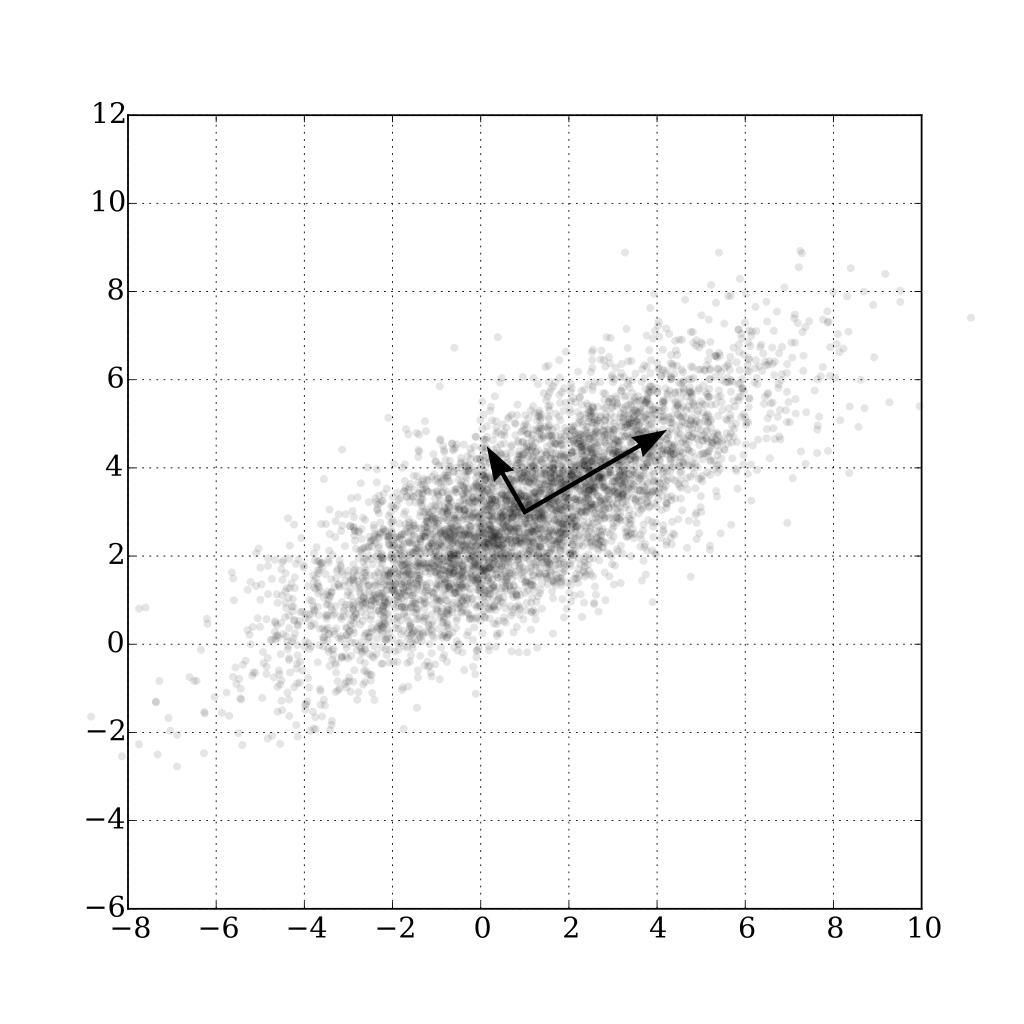
\includegraphics[width=0.4\textwidth]{1024px-GaussianScatterPCA.svg.png}
\end{frame}

\section{Linearization}

\begin{frame}
    \frametitle{State Space Form}

    \begin{equation}
        \diff{t} \bm{x}(t) = f(\bm{x}(t), \bm{u}(t))
    \end{equation}
    But what if \(f(\bm{x}(t), \bm{u}(t))\) isn't linear?
\end{frame}

\begin{frame}
    \frametitle{Linearity}

    Given a system \(y(t) = f(x(t))\),
    \begin{align}
        a x(t) &\iff a y(t) \\
        x_1(t) + x_2(t) &\iff y_1(t) + y_2(t) \\
        a x_1(t) + b x_2(t) &\iff a y_1(t) + b y_2(t)
    \end{align}
\end{frame}

\begin{frame}
    \frametitle{Taylor Approximations}

    Calculus review!
    \begin{align}
        f(x) &= \sum_{n \geqslant 0} \frac{f^{(n)}(x_0)}{n!} (x - x_0)^n = \frac{f(x_0)}{0!} + \frac{f'(x_0)}{1!} (x - x_0) + \frac{f''(x_0)}{2!} (x - x_0)^2 + \cdots \\
        &\approx f(x_0) + f'(x_0) (x - x_0)
    \end{align}
\end{frame}

\begin{frame}
    \frametitle{Linearization}

    \begin{align}
        \bm{J}_{\bm{x}} &=
        \begin{bmatrix}
            \partial_{x_1} f_1 & \partial_{x_2} f_1 & \cdots & \partial_{x_n} f_1 \\
            \partial_{x_1} f_2 & \partial_{x_2} f_2 & \cdots & \partial_{x_n} f_2 \\
            \vdots & \vdots & \ddots & \vdots \\
            \partial_{x_1} f_n & \partial_{x_2} f_n & \cdots & \partial_{x_n} f_n
        \end{bmatrix} \\
        \bm{J}_{\bm{u}} &=
        \begin{bmatrix}
            \partial_{u_1} f_1 & \partial_{u_2} f_1 & \cdots & \partial_{u_n} f_1 \\
            \partial_{u_1} f_2 & \partial_{u_2} f_2 & \cdots & \partial_{u_n} f_2 \\
            \vdots & \vdots & \ddots & \vdots \\
            \partial_{u_1} f_n & \partial_{u_2} f_n & \cdots & \partial_{u_n} f_n
        \end{bmatrix} \\
        \diff{t} \bm{x}(t) &\approx \bm{J}_{\bm{x}} (\bm{x}(t) - \bm{x}^\ast) + \bm{J}_{\bm{u}} (\bm{u}(t) -\bm{u}^\ast)
    \end{align}
\end{frame}

\end{document}
